\documentclass[a4paper, 12pt]{article}
\usepackage{graphicx}
\usepackage[margin=2cm]{geometry}
\usepackage[hidelinks]{hyperref}
\usepackage[croatian]{babel}
\usepackage[sorting=none]{biblatex}
    \addbibresource{ref.bib}
\usepackage{float}

% Boje za kod:
\usepackage{xcolor,graphicx}
\usepackage{listings}

\definecolor{solarized-base03}{RGB}{0, 43, 54}
\definecolor{solarized-base02}{RGB}{7, 54, 66}
\definecolor{solarized-base01}{RGB}{88, 110, 117}
\definecolor{solarized-base00}{RGB}{101, 123, 131}
\definecolor{solarized-base0}{RGB}{131, 148, 150}
\definecolor{solarized-base1}{RGB}{147, 161, 161}
\definecolor{solarized-base2}{RGB}{238, 232, 213}
\definecolor{solarized-base3}{RGB}{253, 246, 227}
\definecolor{solarized-yellow}{RGB}{181, 137, 0}
\definecolor{solarized-orange}{RGB}{203, 75, 22}
\definecolor{solarized-red}{RGB}{220, 50, 47}
\definecolor{solarized-magenta}{RGB}{211, 54, 130}
\definecolor{solarized-violet}{RGB}{108, 113, 196}
\definecolor{solarized-blue}{RGB}{38, 139, 210}
\definecolor{solarized-cyan}{RGB}{42, 161, 198}
\definecolor{solarized-green}{RGB}{133, 153, 0}

\lstset{
  basicstyle=\footnotesize\ttfamily\color{solarized-base00},
  keywordstyle=\color{solarized-blue}\bfseries,
  commentstyle=\color{solarized-base1},
  stringstyle=\color{solarized-cyan},
  identifierstyle=\color{solarized-violet},
  numberstyle=\tiny\color{solarized-base01},
  numbers=left,
  firstnumber=1,
  stepnumber=1,
  showstringspaces=false,
  tabsize=4,
  frame=none,
  framerule=1pt,
  framexleftmargin=5pt,
  framexrightmargin=5pt,
  framextopmargin=3pt,
  framexbottommargin=3pt,
  backgroundcolor=\color{solarized-base3},
  rulecolor=\color{solarized-base01},
  breaklines=true,
  breakatwhitespace=true,
  language=C++
}


\begin{document}
\noindent
Univerzitet u Sarajevu\\
Elektrotehnički fakultet\\
Predmet: Uvod u digitalnu obradu slike\\
Predmetni profesor: prof. dr Emir Sokić\\
Autor: Berina Biberović\\
Akademska godina: 2022/2023.


\begin{center}
    \section*{Tutorijal 9}
    \subsection*{Kalibracija kamere}
\end{center}



Neke kamere prave veliku distorziju prilikom slikanja. Dva generalna tipa distorzije su radijalna i tangencijalna distorzija. Radijalna distorzija utiče na sliku tako što se prave linije čine zakrivljenim - distorzija postaje veća što su pikseli dalje od centra slike. Tangencijalna distorzija se javlja zato što sočivo kamere nije savršeno paralelno sa ravni u kojoj je slika. U tom slučaju, neka područja na slici izgledaju bliža nego očekivano. Za više detalja možete pogledati predavanje 10.

U suštini, potrebno je da izračunamo dvije matrice kako bismo negirali efekat distorzije na slici - jedna je matrica distorzionih koeficijenata, a druga je matrica kamere. Kalibracija kamere predstavlja određivanje ove dvije matrice. Kalkulacija parametara se radi preko osnovnih geometrijskih jednačina. Jednačine zavise od odabranih kalibracijskih objekata. Mi ćemo na ovom tutorijalu naučiti kako da koristimo šahovsku tablu za kalibraciju kamere. Potrebno je uslikati šahovsku tablu kamerom minimalno dva puta kako bismo mogli računati potrebne parametre unutar OpenCV-a. Mi nećemo koristiti samo dvije slike, nego više njih, kako bismo imali što bolje rezultate.

Prvo je potrebno da pronađemo vrhove šahovske table na slici. To možemo uraditi koristeći funkciju \lstinline{bool cv::findChessboardCorners(InputArray slika, Size velicina, OutputArray vrhovi, int flag = cv::CALIB_CB_ADAPTIVE_THRESH+CALIB_CB_NORMALIZE_IMAGE)}. Prvi parametar predstavlja sliku šahovske table (mora biti 8-bitna \textit{grayscale slika} ili slika u boji), drugi parametar predstavlja broj unutrašnjih vrhova po redu i koloni table, treći parametar je izlazni niz detektovanih vrhova, i posljednji parametar predstavlja različite operacijske \textit{flag}-ove koji mogu biti nula ili kombinacija nekih od datih vrijednosti. Nakon toga bi trebalo iscrtati na originalnoj slici gdje su pronađeni vrhovi. Zato što je ovo malo duža procedura koja se treba izvršiti nad svakom slikom koju smo uslikali, bilo bi pametno napraviti funkciju koja će da radi sve što je navedeno.

\begin{lstlisting}
    void PronadjiVrhoveTable(cv::Mat &slika_table, std::vector<cv::Point2f> &vrhovi) {

        // Ovaj parametar predstavlja unutrasnje vrhove table, po redovima i kolonama:
        cv::Size broj_vrhova(x, y);

        // Funkcija za pronalazak vrhova:
        bool pronadjeno = cv::findChessboardCorners(slika_table, broj_vrhova, vrhovi);

        // Ako su uspjesno pronadjeni vrhovi, crtamo vrhove table:
        if(pronadjeno)
            cv::drawChessboardCorners(slika_table, broj_vrhova, cv::Mat(vrhovi), pronadjeno);

        // Sada koristimo instancu klase TermCriteria:
        cv::TermCriteria termcrit(cv::TermCriteria::COUNT|cv::TermCriteria::EPS, 20, 0.03);
        // Prethodnu varijablu iskoristimo u funkciji cv::cornerSubPix kako bismo nasli vise egzaktne pozicije vrhova:
        cv::cornerSubPix(slika_table, vrhovi, cv::Size(11, 11), cv::Size(-1, -1), termcrit);
        
    }
\end{lstlisting}

Prethodna funkcija predstavlja način kako se može implementirati pronalazak vrhova na šahovskoj tabli. Primijetimo da u liniji 4 varijabla \lstinline{broj_vrhova} je inicijalizirana na \lstinline{x, y} - objasnili smo ranije da ovaj parametar predstavlja broj unutrašnjih vrhova po redu i koloni šahovske table, dakle, potrebno ga je mijenjati na osnovu slika šahovske table koje imate. Možete izmijeniti prethodnu funkciju tako da se svaki put šalju parametri \lstinline{(x, y)}, a možete samo staviti da su to brojevi unutar funkcije ukoliko znate da ste slikali istu šahovsku tablu više puta iz više uglova. 

Primijetimo pored toga da su parametri koje prima naša funkcija \lstinline{PronadjiVrhoveTable} poslani kao reference - to je urađeno da se smanji količina kopiranja podataka iz \lstinline{main} funkcije, a pored štednje memorije štedimo i na brzini u tom slučaju. Prvi parametar koji prima naša funkcija je ustvari slika šahovske table, dok je drugi parametar vektor tačaka u koji ćemo upisati pronađene vrhove.

Dalje, u liniji 7 koristimo gotovu funkciju iz OpenCV-a o kojoj smo maloprije pričali kako bismo našli vrhove table, \lstinline{cv::findChessboardCorners}. Ukoliko su uspješno pronađeni vrhovi (linija 10), onda crtamo vrhove preko gotove funkcije \lstinline{cv::drawChessboardCorners} kojoj šaljemo sliku šahovske table, varijablu koja predstavlja broj unutrašnjih vrhova table po redu i po koloni, pronađeni vektor tačaka vrhova iz prethodne funkcije koji smo automatskom pretvorbom pretvorili u \lstinline{cv::Mat} tip i na kraju \lstinline{bool} koji govori je li uspješno prošao pronalazak vrhova. Sada je slika šahovske table izmijenjena i sadrži kružiće na svim pronađenim vrhovima.

\lstinline{cv::findChessboardCorners} daje dovoljno dobre rezultate za ljudsko oko, no ona ćoškove samo aproksimativno nalazi. Pošto je cilj kalibracija kamere potrebno je da lokacije ovih vrhova budu što preciznije određene.

Iz tog razloga, koristimo sljedeću funkciju \lstinline{cv::cornerSubPix} koja nam omogućava da nađemo \textit{sub-pixel} tačnu lokaciju vrhova, u ovom slučaju, šahovske table. Dakle, ova funkcija poboljšava lokacije vrhova. Da bismo je koristili, potrebna nam je instanca klase \lstinline{cv::TermCriteria} koja u svom konstruktoru prima tri parametra: tip terminacijskog kriterija, maksimalan broj iteracija ili maksimalan broj elemenata za računanje i epsilon tj. željenu preciznost pri kojoj iterativni algoritam se zaustavlja.

U našoj funkciji smo stavili da je prvi tip parametra dva navedene \lstinline{enum} tipa sa \textit{bitwise or} operatorom (možete detaljnije pronaći šta znače ova dva \lstinline{enum} tipa na \href{https://docs.opencv.org/4.x/d9/d5d/classcv_1_1TermCriteria.html#a56fecdc291ccaba8aad27d67ccf72c57}{linku}). Za drugi parametar smo stavili da algoritam \lstinline{cv::cornerSubPix} zaustavi algoritam nakon 20 iteracija, a za treći parametar da se zaustavi nakon što promjena epsilon bude manja ili jednaka 0.03.

Nakon toga, pozivamo funkciju \lstinline{cv::cornerSubPix} kojoj prosljeđujemo sliku šahovske table, niz do sada pronađenih vrhova u koji će se upisati preciznije lokacije vrhova, pola dužine prozora koji pretražuje sliku (u ovom slučaju je \lstinline{cv::Size(11, 11)} što znači da se koristi prozor veličine $23 \times 23$), pola veličine mrtve zone u sredini zone pretraživanja gdje se sumacija u formuli za pretraživanje ne radi (kod nas je taj parmetar jednak \lstinline{cv::Size(-1, -1)}, što znači da ne postoji takva veličina u našem slučaju) i na kraju kriterij koji smo prethodno inicijalizirali i objasnili.

Nakon cijele ove procedure imamo lokaciju vrhova na šahovskoj tabli! Ali to nije dovoljno za kalibraciju kamere - pogledajmo funkciju \lstinline{cv::calibrateCamera} koju trebamo iskoristiti da bismo izračunali matricu kamere, koeficijente distance, rotacijski vektor i translacijski vektor - sve informacije koje su nam potrebne za kalibraciju.

Funkcija \lstinline{cv::calibrateCamera} koju ćemo mi koristiti je preklopljena funkcija članica koja prima 9 parametara (originalna prima 12). Razlog zašto koristimo preklopljenu funkciju članicu je što mi nemamo sve koeficijente za napredno kalibrisanje kamere, koje originalna funkcija traži. Prototip ove funkcije glasi:

\begin{lstlisting}
    double cv::calibrateCamera(InputArrayOfArrays tacke_objekta, InputArrayOfArrays tacke_slike, Size velicina_slike, InputOutputArray matrica_kamere, InputOutputArray koeficijenti_distance, OutputArrayOfArrays rotacijski_vektor, OutputArrayOfArrays translacijski_vektor, int flag = 0, TermCriteria kriterij = TermCriteria(TermCriteria::COUNT+TermCriteria::EPS, 30, DBL_EPSILON))
\end{lstlisting}

Kao što možemo vidjeti, ovo je stvarno velika funkcija. Sve parametre imamo, osim parametra \lstinline{tacke_objekta}. Taj parametar će kod nas biti tipa \lstinline{std::vector<std::vector<cv::Point3f>>} i predstavlja vektor vektora tačaka kalibracijskog šablona u koordinacijskom prostoru kalibracijskog obrasca. Šta uopšte ovo znači za nas? Pojednostavljeno, veliki vektor ima broj elemnata onoliko koliko ima slika koje koristimo za kalibraciju i u našem slučaju svaki taj vektor je isti! U detalje kad i zašto ne moraju biti ovi vektori isti nećemo ulaziti. Razlog zašto su ovi elementi isti je što će kod nas set slika za kalibraciju (koji ćete dobiti na laboratorijskoj vježbi) uvijek sadržavati šahovsku tablu bez opstrukcija ili zaklanjanja, dakle tabla je uvijek u potpunosti vidljiva na slici. Način na koji ćemo inicijalizirati ovaj vektor je sljedeći:

\begin{lstlisting}
    for(int k = 0; k < broj_slika_za_kalibraciju; k++)
        for(int i = 0; i < y; i++)
            for(int j = 0; j < x; j++)
                tacke_objekta.at(k).push_back(cv::Point3f(j, i, 0));
\end{lstlisting}

Sjetimo se šta parametri \lstinline{(x, y)} znače - broj unutrašnjih ivica šahovske table po redu i po koloni.

Dalje, parametar \lstinline{tacke_slike} je tipa \lstinline{std::vector<std::vector<cv::Point2f>>} i predstavlja sve ivice koje smo našli prethodno koristeći funkciju \lstinline{PronadjiVrhoveTable}. Veliki vektor u ovom slučaju sadrži vektore ivica šahovskih ploča sa svih slika iz seta za kalibraciju.

Parametar \lstinline{velicina_slike} je tipa \lstinline{cv::Size} i dovoljno je uzeti jednu sliku iz seta za kalibraciju, učitati je u objekat tipa \lstinline{cv::Mat} i inicijalizirati ovaj parametar kao \lstinline{cv::Size(slika.rows, slika.cols)}, gdje je \lstinline{slika} spomenuta učitana slika.

Parametri \lstinline{matrica_kamere}, \lstinline{koeficijenti_distance}, \lstinline{rotacijski_vektor} i \lstinline{translacijski_vektor} su svi tipa \lstinline{cv::Mat}. Njih ne moramo uopšte inicijalizirati jer će njihova vrijednost biti izračunata pozivom funkcije \lstinline{cv::calibrateCamera}. Posljednja dva parametra ne moramo uopšte slati jer su oni preklopljeni.

Nakon cijele ove procedure, dobili smo tražene matrice za kalibraciju kamere. Ukoliko želimo da prikažemo sada sliku koja nema distorzije na sebi, možemo koristiti funkciju \lstinline{cv::undistort} koja prima sljedeće parametre: izvornu sliku koja ima distorzije u sebi, sliku u koju ćemo sačuvati rezultat funkcije nakon uklanjanja distorzije, prethodno izračunatu matricu \lstinline{matrica_kamere} i koeficijente distance \lstinline{koeficijenti_distance}. 

Da bismo pokazali kako radi \lstinline{cv::undistort}, na slici \ref{sl1} je prikazana originalna slika, dok je na slici \ref{sl2} prikazana slika sa uklonjenom distorzijom. Kao što možemo vidjeti, ukanjanje distorzije nije savršeno prošlo, ali svakako na slici  \ref{sl2} šahovska tabla puno bolje izgleda i vidno ima puno manje distorzije od slike \ref{sl1}, ali pošto smo kalibrisali kameru na osnovu šahovske table, vidimo da pozadina na slici \ref{sl2} je iskrivljena.

\begin{figure}[H]
    \centering
    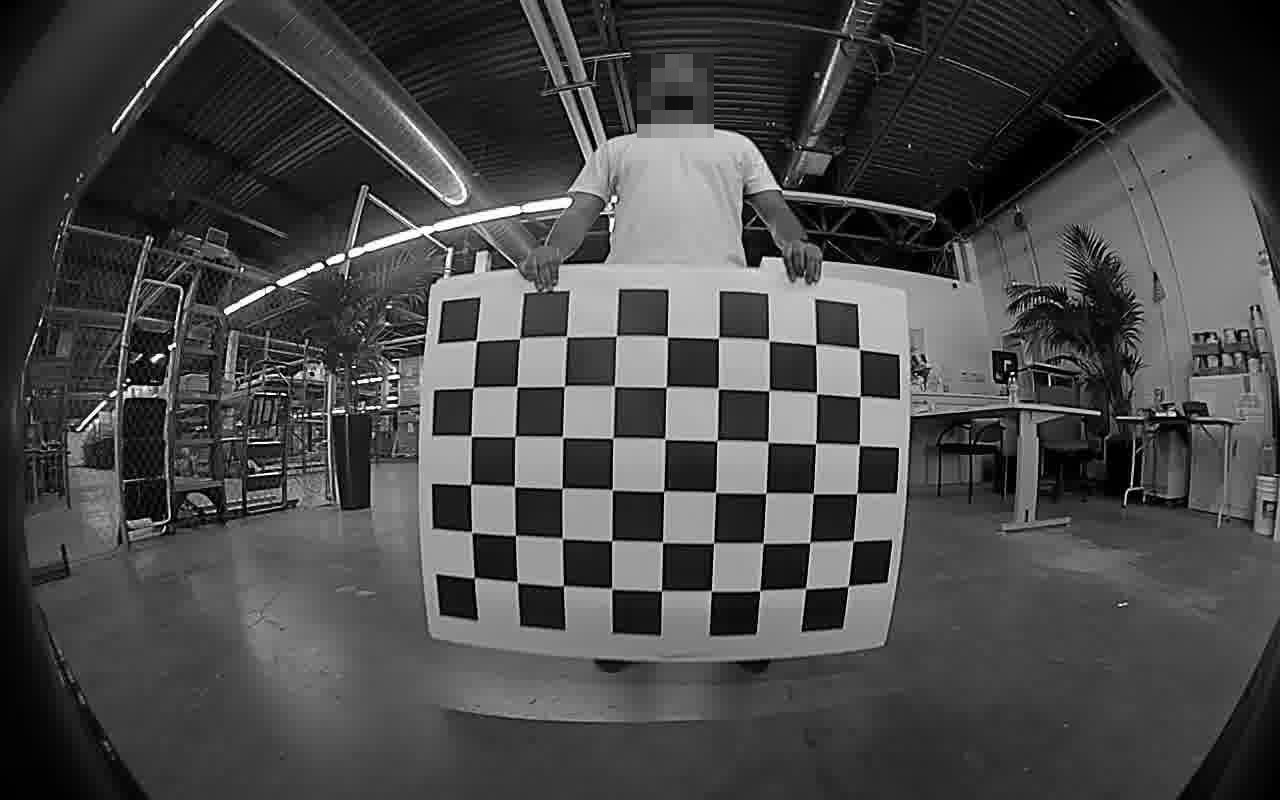
\includegraphics[width=\textwidth]{Slike/original.jpg}
    \caption{Originalna slika}
    \label{sl1}
\end{figure}

\begin{figure}[H]
    \centering
    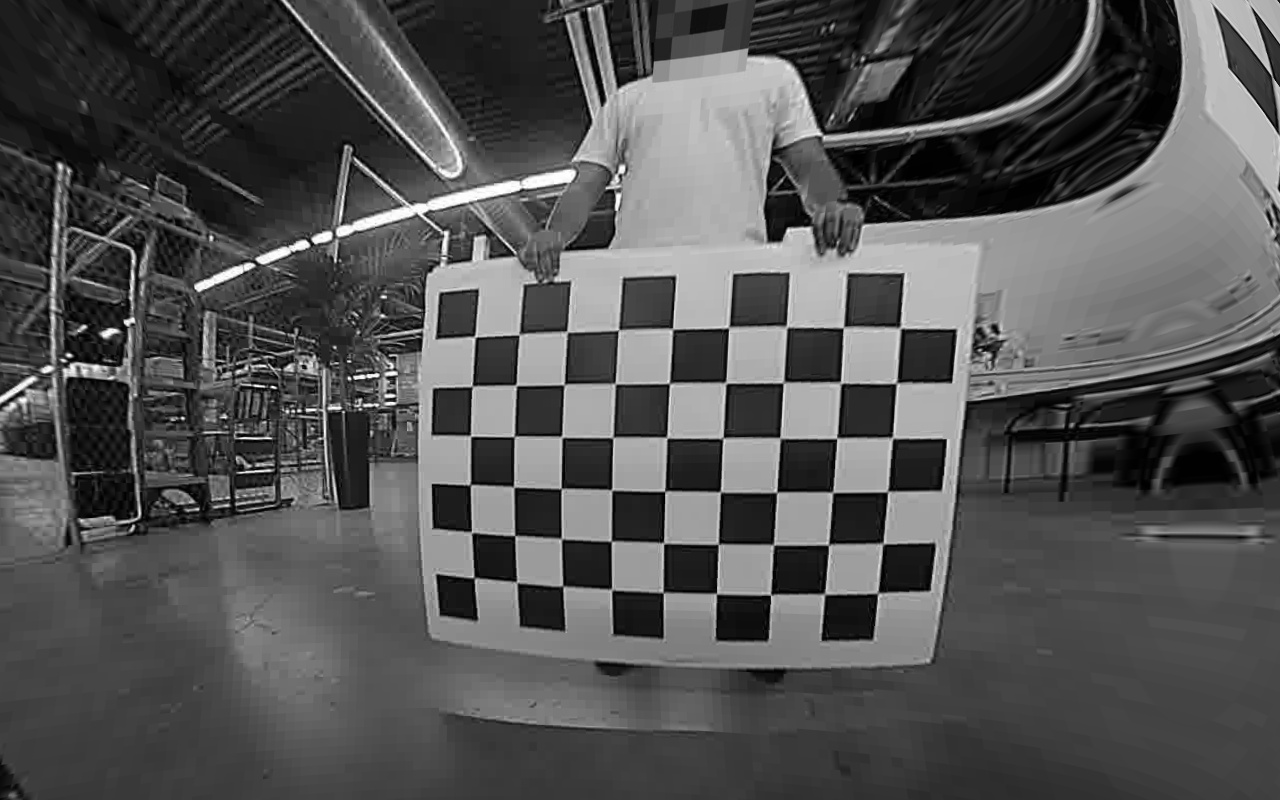
\includegraphics[width=\textwidth]{Slike/bez_distorzije.jpg}
    \caption{Slika nakon primjenjivanja \lstinline{cv::undistort} funkcije}
    \label{sl2}
\end{figure}

\subsection*{Napomene}

Korištena tema za prikaz C++ koda na tutorijalima je \href{https://ethanschoonover.com/solarized/}{\lstinline{solarized}}\cite{solarized}.

\printbibliography

\end{document}
